\documentclass[11pt]{article}
\usepackage[a4paper,left=25mm,right=25mm,top=24mm,bottom=25mm,headheight=14pt]{geometry}
\usepackage{amsmath,amssymb,amsthm,booktabs,float,algorithm,algpseudocode}
\usepackage{graphicx,array,microtype}
\usepackage[T1]{fontenc}
\usepackage{mathpazo,titlesec,fancyhdr,caption,enumitem,etoolbox}
\linespread{1.045}
\setlength{\parindent}{1.2em}
\setlength{\parskip}{2pt}
\titleformat{\section}{\large\sffamily\bfseries}{\thesection}{0.65em}{}
\titleformat{\subsection}{\normalsize\sffamily\bfseries}{\thesubsection}{0.65em}{}
\titlespacing*{\section}{0pt}{2.0ex plus 1ex minus .2ex}{1.1ex}
\titlespacing*{\subsection}{0pt}{1.6ex plus .5ex}{0.7ex}
\captionsetup{font=small,labelfont=bf,labelsep=period,skip=8pt}
\setlist[enumerate]{leftmargin=1.8em,itemsep=4pt,topsep=6pt}
\pagestyle{fancy}
\fancyhf{}
\fancyhead[L]{\small\itshape Complex-corrected stochastic gradient descent}
\fancyfoot[C]{\small\thepage}
\renewcommand{\headrulewidth}{0pt}
\AtBeginEnvironment{thebibliography}{\small}
\renewcommand{\maketitle}{%
  \thispagestyle{plain}%
  \begingroup\raggedright
  {\fontsize{22}{26}\selectfont\bfseries
  Complex-Corrected\\Stochastic Gradient Descent\\for Noisy Observations\par}
  \vspace{12pt}\hrule\vspace{14pt}
  \endgroup}
\renewenvironment{abstract}
  {\small\noindent\textbf{Abstract.}\ignorespaces}
  {\par\vspace{10pt}}
\usepackage[hidelinks]{hyperref}
\floatstyle{ruled}\restylefloat{algorithm}
\setlength{\tabcolsep}{4pt}
\setlength{\emergencystretch}{1em}
\raggedbottom
\numberwithin{equation}{section}
\newtheoremstyle{emphasizedplain}
  {9pt plus 2pt minus 1pt}{9pt plus 2pt minus 1pt}
  {\itshape}{}{\bfseries}{.}{0.6em}
  {\thmname{#1}\thmnumber{ #2}\thmnote{\textbf{ (#3)}}}
\newtheoremstyle{emphasizeddefinition}
  {9pt plus 2pt minus 1pt}{9pt plus 2pt minus 1pt}
  {\normalfont}{}{\bfseries}{.}{0.6em}
  {\thmname{#1}\thmnumber{ #2}\thmnote{\textbf{ (#3)}}}
\theoremstyle{emphasizedplain}
\newtheorem{theorem}{Theorem}[section]
\newtheorem{lemma}[theorem]{Lemma}
\theoremstyle{emphasizeddefinition}
\newtheorem{assumption}[theorem]{Assumption}
\title{Complex-Corrected Stochastic Gradient Descent for Noisy Observations}
\author{}
\date{}
\hypersetup{pdftitle={Complex-Corrected Stochastic Gradient Descent for Noisy Observations},
pdfsubject={Exact gradient correction and stochastic optimization under Gaussian measurement error}}
\begin{document}
\maketitle
\begin{abstract}
We study stochastic optimization with Gaussian measurement error in the
inputs. For scores admitting an entire extension, complex-corrected
stochastic gradient descent evaluates the score at a noisy observation
plus an independent imaginary Gaussian perturbation. Building on the
classical complex corrected-score identity, this gives a directly
implementable learning rule whose gradient is exactly unbiased at every
iteration, rather than corrected only to finite order. Under an exponential
derivative bound with parameter-dependent amplitude, a gradient-based
amplitude control, and sub-Gaussian latent inputs, we derive the conditional
moment estimates that place this recursion within classical stochastic
approximation. We obtain convex objective bounds, almost-sure convergence
to the clean optimizer $\theta^*$ and mean-square rates under strong
convexity, and nonconvex stationarity bounds. We also establish
last-iterate and averaged central limit laws for step sizes
$c/(t+\gamma)^\alpha$, $1/2<\alpha\le1$, including the distinct averaging
covariance at $\alpha=1$. The construction allows any known positive
semidefinite noise covariance. We discuss exact correction for admissible
non-Gaussian errors, including uniform and symmetric two-point noise,
under suitable integrability conditions. Explicit examples and numerical
experiments illustrate parameter convergence and improved prediction
over naive training.
\end{abstract}

\section{Introduction}

Consider the stochastic optimization problem
\[
\min_{\theta\in\mathbb R^p}F(\theta),\qquad
F(\theta)=\mathbb E\ell(\theta;Z),
\]
when the latent input $Z$ is observed only through $W=Z+U$.
Even for centered measurement error, the score
$g(\theta;W)=\nabla_\theta\ell(\theta;W)$ is generally biased for
$\nabla F(\theta)$. A decreasing step size controls stochastic
fluctuations but does not eliminate this discrepancy. The question is
whether noisy observations can nevertheless support an explicit
stochastic-gradient method for the clean objective.

For Gaussian error with known covariance, the classical complex
corrected-score identity provides a construction
\cite{stefanski1989,novick2002}. If the score has an integrable entire
extension, an independent imaginary Gaussian perturbation cancels the
measurement error in expectation. This leads to complex-corrected
stochastic gradient descent (CCSGD):
\[
\theta_{t+1}=\theta_t-\eta_t\operatorname{Re}
g^{\mathbb C}(\theta_t;W_t+iV_t),\qquad
V_t\sim N(0,\Omega).
\]
Each iteration uses one noisy observation and one complex score evaluation.
Only the noise covariance is required; it may be correlated or singular.

The central analytical issue is control of the corrected gradient along
the stochastic trajectory. Pointwise unbiasedness and finite variance
do not by themselves give the conditional moment bounds required for
convergence. We address this issue through three results.
\begin{enumerate}
\item \emph{Exact correction.}
We formulate the Gaussian correction for vector-valued entire scores
under an explicit exponential growth condition. The construction is
independent of the convexity of the objective.
\item \emph{Relative variance control.}
We bound the correction error using the score's input derivative and
the tails of the latent and Gaussian variables. The derivative amplitude
may grow with the parameter, provided its square is controlled by the
squared objective gradient. Conditional orthogonality then yields the
classical SGD relative variance condition and local higher-moment control
for limit laws.
\item \emph{Convergence and fluctuations.}
For polynomially decaying step sizes with exponent $1/2<\alpha\le1$,
we establish convex objective bounds, strongly convex mean-square rates
and almost-sure convergence, and nonconvex stationarity bounds.
Under local regularity, we identify the last-iterate and averaged
Gaussian limits, including the $\alpha=1$ endpoint.
\end{enumerate}
The analysis connects the classical Gaussian identity to stochastic
approximation through explicit moment estimates
\cite{novick2002,fabian1968,polyakjuditsky1992}. Examples and numerical
studies illustrate the method; a separate moment argument covers
nonlinear-feature regression.

\section{Related work}
\label{sec:related_work}

\begin{table}[H]
\centering
\small
\caption{Selected approaches to measurement-error correction. Exactness is understood within each method's stated model and function class.}
\label{tab:related_work}
\renewcommand{\arraystretch}{1.08}
\begin{tabular}{>{\raggedright\arraybackslash}p{0.23\linewidth}>{\raggedright\arraybackslash}p{0.34\linewidth}>{\raggedright\arraybackslash}p{0.35\linewidth}}
\toprule
Work & Main result & Relation to CCSGD \\
\midrule
Nakamura (1990) \cite{nakamura1990} & Corrected estimating equations & Foundational score-correction principle. \\
Novick--Stefanski (2002) \cite{novick2002} & Exact Gaussian complex Monte Carlo corrected scores and batch $M$-estimation & Our Gaussian correction uses their identity; we study its per-sample use in SGD. \\
Stefanski (1989) \cite{stefanski1989} & Analyticity restriction for globally unbiased Gaussian correction & Delimits exact correction for scores with complex singularities. \\
Konstantopoulos--Patie--Sarkar (2024) \cite{konstantopoulos2024} & van Dantzig pairs and distributional constructions & Supplies candidate conjugate perturbations for non-Gaussian noise; score integrability remains to be checked. \\
Woolsey--Huang (2026) \cite{woolseyhuang2026} & Statistical estimation with non-Gaussian error through finite-order bias cancellation & CCSGD gives an explicit stochastic-gradient update and optimization guarantees; exact correction for admissible non-Gaussian noise is discussed in Further work. \\
Cook--Stefanski (1994); Spicker et al. (2024) \cite{cookstefanski1994,spicker2024} & Parametric and nonparametric SIMEX & Correct by extrapolation rather than an exact per-sample gradient identity. \\
Belomestny--Goldenshluger (2021) \cite{belomestnygoldenshluger2021} & Density deconvolution allowing zeros of the error characteristic function & Related inverse problem; its target is density estimation. \\
Loh--Wainwright (2012) \cite{lohwainwright2012} & Corrected high-dimensional sparse linear regression with a convergent projected-gradient algorithm & Addresses linear regression; CCSGD treats scores of more general analytic losses in an online stochastic update. \\
Carroll et al. (2006) \cite{carroll2006} & Regression calibration and broader measurement-error methodology & Context for plug-in correction. \\
\bottomrule
\end{tabular}
\end{table}

Nakamura's corrected-score principle and the complex Monte Carlo
construction of Novick and Stefanski \cite{nakamura1990,novick2002}
provide the statistical foundation. CCSGD studies the associated online
gradient recursion and derives its noise conditions before applying
classical optimization theory. Loh and Wainwright
\cite{lohwainwright2012} already provide a computationally tractable
corrected optimization method for sparse linear regression; our analysis
allows more general analytic scores under explicit growth conditions.
Woolsey and Huang \cite{woolseyhuang2026} develop non-Gaussian
corrections for statistical estimation by cancelling finitely many bias
terms, which generally leaves a residual bias. Our focus is stochastic
optimization: CCSGD gives a directly implementable learning rule using
one noisy observation and one simulated complex perturbation per update,
with convergence rates and asymptotic guarantees. Further work discusses
exact correction for non-Gaussian noise admitting a suitable conjugate
perturbation, including uniform and symmetric two-point noise, under the
required score-integrability conditions. In our experiments, the
Woolsey--Huang baseline is their deterministic correction in Eq.~(5).

\subsection*{Our contributions}
\begin{enumerate}
\item \emph{An explicit optimization method.}
CCSGD turns complex correction into a directly implementable stochastic
optimization algorithm for a broad class of analytic losses with noisy
inputs. Each update evaluates the score at one noisy observation plus
one simulated complex perturbation. Experiments demonstrate convergence
to the true parameter in nonlinear-feature regression and improved
prediction over naive training in neural-network regression.
\item \emph{Exact correction beyond Gaussian noise.}
The conjugate-variable criterion in our companion work
\cite{conjugatecriterion2026} extends the correction principle to
admissible non-Gaussian noise, including uniform and symmetric two-point
distributions. Further work describes these constructions and the
integrability conditions required for exact unbiasedness; the main
optimization theorems here concern Gaussian measurement error.
\item \emph{Per-step unbiasedness and asymptotic guarantees.}
The corrected gradient is exactly unbiased at every iteration, rather
than merely cancelling finitely many bias terms. We derive the classical
SGD relative variance bound from input growth and sampling conditions,
then establish convex and nonconvex guarantees. Under strong convexity,
CCSGD converges to the clean optimizer $\theta^*$ almost surely and in
mean square, with explicit MSE rates; under the stated local regularity
conditions, both the last iterate and the Polyak--Ruppert average are
asymptotically normal.
\end{enumerate}

\section{Complex-Corrected SGD}
\label{sec:algorithm}

Let $\theta\in\mathbb R^p$. A fixed response, when present, is suppressed in the notation. We observe $W=Z+U$, where $U\sim N(0,\Omega)$ is independent of $Z$ and the covariance $\Omega\succeq0$ is known. No invertibility or diagonal structure is required. Assume that $Z\in\mathbb R^d$ is sub-Gaussian about its mean $m_Z$: for some $\sigma_Z<\infty$,
\[
\mathbb E e^{s v^\top(Z-m_Z)}\le e^{\sigma_Z^2s^2/2}
\quad(s\in\mathbb R,\ \|v\|=1).
\]
For a loss $\ell(\theta;z)$ differentiable in $\theta$, with
$\mathbb E|\ell(\theta;Z)|<\infty$ for every $\theta$, write
\[
F(\theta)=\mathbb E_Z\ell(\theta;Z),\qquad
g(\theta;z)=\nabla_\theta\ell(\theta;z).
\]
The following assumptions separate input regularity from clean sampling
noise. All norms are Euclidean, with $\|\cdot\|_{\rm op}$ denoting the
induced operator norm.

\begin{assumption}[Holomorphic score]\label{ass:entire}
For every $\theta$, $z\mapsto g(\theta;z)$ admits an entire extension $g^{\mathbb C}(\theta;\cdot)$ on $\mathbb C^d$, real-valued on $\mathbb R^d$.
\end{assumption}

\begin{assumption}[Exponential envelope]\label{ass:envelope}
There are a finite constant $a\ge0$ and a measurable function
$M:\mathbb R^p\to[0,\infty)$ such that
\begin{equation}\label{eq:parameter_envelope}
\|D_qg^{\mathbb C}(\theta;q)\|_{\rm op}
\le M(\theta)e^{a\|q\|},
\qquad \theta\in\mathbb R^p,\ q\in\mathbb C^d.
\end{equation}
The exponent $a$ is independent of $\theta$; the amplitude $M(\theta)$
need not be bounded.
In addition, for finite constants $A,B\ge0$,
\begin{equation}\label{eq:amplitude_control}
M(\theta)^2\le A+B\|\nabla F(\theta)\|^2,
\qquad \theta\in\mathbb R^p.
\end{equation}
\end{assumption}

\begin{assumption}[Clean sampling variance]\label{ass:clean_variance}
Differentiation may be interchanged with the expectation defining $F$,
and for constants $\sigma_0^2,\rho_0\ge0$, independent of $\theta$,
\[
\mathbb E_Z\|g(\theta;Z)-\nabla F(\theta)\|^2
\le\sigma_0^2+\rho_0\|\nabla F(\theta)\|^2.
\]
This condition concerns the clean stochastic score;
no variance bound is assumed on the corrected score.
\end{assumption}

The amplitude control transfers the input growth bound to the standard
SGD relative variance condition. The correction identity itself uses
only the entire extension and the bound~\eqref{eq:parameter_envelope};
it requires neither amplitude control nor convexity.

\begin{algorithm}[H]
\caption{Complex-Corrected SGD}
\label{alg:ccsgd}
\begin{algorithmic}[1]
\Require Initial point $\theta_1$, step sizes $\{\eta_t\}_{t=1}^T$, known noise covariance $\Omega$
\For{$t=1,\ldots,T$}
    \State Observe a fresh $W_t=Z_t+U_t$
    \State Draw $V_t\sim N(0,\Omega)$ independently of the observation and the past
    \State $G_t\gets\operatorname{Re}g^{\mathbb C}(\theta_t;W_t+iV_t)$
    \State $\theta_{t+1}\gets\theta_t-\eta_tG_t$
\EndFor
\State \Return $\theta_{T+1}$
\end{algorithmic}
\end{algorithm}

\paragraph{Optional averaging.}
For the same observation $W_t$, one may draw $m$ independent
$V_{t,j}\sim N(0,\Omega)$ and replace $G_t$ by
\[
G_t^{(m)}=\frac1m\sum_{j=1}^m
\operatorname{Re}g^{\mathbb C}(\theta_t;W_t+iV_{t,j}).
\]
This preserves conditional unbiasedness with respect to the past.
Given $(\mathcal F_{t-1},W_t)$, the covariance is $1/m$ times that of
a single draw, reducing simulation variability and stabilizing the update
at the cost of additional score evaluations. Variability due to the
shared observation remains.

\begin{lemma}[Exact correction]\label{lem:exact_correction}
Under Assumptions~\ref{ass:entire}--\ref{ass:envelope}, for every $(z,\theta)$,
\[
\mathbb E_{U,V}\bigl[\operatorname{Re}g^{\mathbb C}(\theta;z+U+iV)\bigr]
=g(\theta;z).
\]
Consequently, if $\theta_t$ is measurable with respect to the past $\mathcal F_{t-1}$, $(Z_t,U_t,V_t)$ is independent of that past, and differentiation may be interchanged with the expectation defining $F$, then
$\mathbb E[\operatorname{Re}g^{\mathbb C}(\theta_t;W_t+iV_t)\mid\mathcal F_{t-1}]=\nabla F(\theta_t)$.
\end{lemma}


\paragraph{Observed responses.}
For noise-free responses $Y=r(Z)$, keep $Y$ fixed when extending
$z\mapsto g(\theta;z,Y)$ to complex inputs. The same argument gives
\[
\mathbb E_{U,V}[\operatorname{Re}g^{\mathbb C}(\theta;Z+U+iV,Y)
\mid Z,Y]=g(\theta;Z,Y),
\]
provided the score satisfies the entire and growth conditions at each
fixed $(\theta,y)$. For the objective
$F(\theta)=\mathbb E\ell(\theta;Z,Y)$, sampling and moment conditions
must hold for the joint pair $(Z,Y)$.
Appendix~\ref{app:regression} derives these bounds for the regression
experiment.

\section{Main results}
\label{sec:main_results}

Throughout this section, the assumptions of Section~\ref{sec:algorithm}
hold. The initial point is deterministic, and $(Z_t,U_t,V_t)$ are i.i.d.
triples, independent of the past $\mathcal F_{t-1}$. Write
$\mathbb E_t[\cdot]=\mathbb E[\cdot\mid\mathcal F_{t-1}]$ and
\[
\Delta_t=G_t-g(\theta_t;Z_t),\qquad
\xi_t=G_t-\nabla F(\theta_t).
\]
Exact correction gives $\mathbb E_t\xi_t=0$. The exponential envelope and
independence of the fresh data imply
\[
\mathbb E_t\|\Delta_t\|^2\le K_aM(\theta_t)^2
\le K_aA+K_aB\|\nabla F(\theta_t)\|^2,
\]
where
\[
K_a=\mathbb E e^{2a\|Z\|}\,
\mathbb E\!\left[\|U+iV\|^2e^{2a\|U+iV\|}\right]<\infty.
\]
Since $\mathbb E[\Delta_t\mid\mathcal F_{t-1},Z_t]=0$, the cross term vanishes.
Assumption~\ref{ass:clean_variance} therefore yields
\begin{equation}\label{eq:relative_variance}
\mathbb E_t\|\xi_t\|^2
=\mathbb E_t\|\Delta_t\|^2+
\mathbb E_t\|g(\theta_t;Z_t)-\nabla F(\theta_t)\|^2
\le\sigma^2+\rho\|\nabla F(\theta_t)\|^2,
\end{equation}
with
\[
\sigma^2=\sigma_0^2+K_aA,\qquad \rho=\rho_0+K_aB.
\]
These constants are independent of $t$ and $\theta$. Thus the correction
preserves the classical relative variance structure without requiring
a bounded amplitude $M$. All proofs, including the local higher-moment
estimates for the CLTs, are given in Appendix~\ref{app:proofs}.

\paragraph{Mini-batching and Monte Carlo averaging.}
With $n$ independent fresh observations and $m$ independent imaginary
perturbations per observation, use
\[
G_t^{(n,m)}=\frac1n\sum_{i=1}^n\frac1m\sum_{j=1}^m
\operatorname{Re}g^{\mathbb C}(\theta_t;W_{t,i}+iV_{t,i,j}).
\]
All perturbations are independent of the observations and the past.
For fixed $\theta$, write
$h_\theta(W)=\mathbb E_V[\operatorname{Re}g^{\mathbb C}(\theta;W+iV)\mid W]$
and define
\[
\begin{aligned}
v_{\rm obs}(\theta)&=\mathbb E\|h_\theta(W)-\nabla F(\theta)\|^2,\\
v_{\rm sim}(\theta)&=\mathbb E\|G(\theta)-h_\theta(W)\|^2.
\end{aligned}
\]
Conditional centering makes the observation and simulation errors
orthogonal. Independence across observations and simulations therefore gives
\begin{equation}\label{eq:batch_mc_variance}
\mathbb E_t\|G_t^{(n,m)}-\nabla F(\theta_t)\|^2
=\frac{v_{\rm obs}(\theta_t)}n+
\frac{v_{\rm sim}(\theta_t)}{nm}
\le\frac{\sigma^2+\rho\|\nabla F(\theta_t)\|^2}{n},
\end{equation}
since $v_{\rm obs}+v_{\rm sim}=\mathbb E\|G-\nabla F\|^2$.
Thus mini-batching reduces both components by $n$, while repeated imaginary
perturbations further reduce only the simulation component by $m$.
The bounds below apply with variance constants $\sigma^2/n$ and $\rho/n$;
for the CLTs, the corrected-oracle covariance is that of $G^{(n,m)}$
when $n$ and $m$ are fixed.
The analysis below requires only the relative variance bound; its precise
constants affect the quantitative bounds, but not the stated convergence
rates or the validity of the CLTs. Averaging is primarily a practical
option for reducing variability and improving training stability.

\begin{theorem}[Convex objective]\label{thm:convex}
Suppose $F:\mathbb R^p\to\mathbb R$ is convex and $L$-smooth and has a
minimizer $\theta^*$. Let $\eta_t=c/(t+\gamma)^\alpha$ with
$c>0$, $\gamma\ge0$, $1/2<\alpha\le1$, and $\eta_1\le1/[L(1+\rho)]$. Define
$\bar\theta_T^{\eta}=(\sum_{t=1}^T\eta_t\theta_t)/
(\sum_{t=1}^T\eta_t)$. Then
\[
\mathbb E[F(\bar\theta_T^{\eta})]-F(\theta^*)
\le
\frac{\|\theta_1-\theta^*\|^2
+\sigma^2\sum_{t=1}^T\eta_t^2}
{2\sum_{t=1}^T\eta_t}.
\]
Consequently, the expected objective gap is $O(T^{\alpha-1})$ if
$\alpha<1$, and $O(1/\log T)$ if $\alpha=1$.
\end{theorem}

\begin{theorem}[Strong convexity]
\label{thm:strong_convex}
Suppose $F:\mathbb R^p\to\mathbb R$ is $\mu$-strongly convex and
$L$-smooth, with minimizer $\theta^*$. Let
$\eta_t=c/(t+\gamma)^\alpha$ with $c>0$, $\gamma\ge0$, and
$1/2<\alpha\le1$. Then $\theta_t\to\theta^*$ almost surely and in
mean square. For $\alpha<1$,
\[
\mathbb E\|\theta_t-\theta^*\|^2=O(t^{-\alpha}).
\]
For $\alpha=1$,
\[
\mathbb E\|\theta_t-\theta^*\|^2=
\begin{cases}
O(t^{-1}), & 2\mu c>1,\\
O(t^{-1}\log t), & 2\mu c=1,\\
O(t^{-2\mu c}), & 2\mu c<1.
\end{cases}
\]

\end{theorem}

For the two central limit theorems, write
\[
S(\theta)=\mathbb E\bigl[(G(\theta)-\nabla F(\theta))
(G(\theta)-\nabla F(\theta))^\top\bigr],\qquad
G(\theta)=\operatorname{Re}g^{\mathbb C}(\theta;Z+U+iV).
\]

\begin{theorem}[Last-iterate fluctuations]\label{thm:last_clt}
In addition to the strong convexity and smoothness conditions of
Theorem~\ref{thm:strong_convex}, suppose $F$ is twice continuously
differentiable near $\theta^*$, its Hessian is locally Lipschitz there,
and $S(\theta)\to S_*:=S(\theta^*)$ as $\theta\to\theta^*$.
Let $H=\nabla^2F(\theta^*)$ and
$\eta_t=c/(t+\gamma)^\alpha$, where $c>0$, $\gamma\ge0$, and
$1/2<\alpha\le1$. If $\alpha<1$, then
\[
t^{\alpha/2}(\theta_t-\theta^*)\ \Rightarrow\ N(0,\Sigma_c),
\qquad H\Sigma_c+\Sigma_c H=cS_*.
\]
If $\alpha=1$ and $c\lambda_{\min}(H)>1/2$, then
\[
\sqrt t\,(\theta_t-\theta^*)\ \Rightarrow\ N(0,\Sigma_c),
\qquad
(cH-\tfrac12 I)\Sigma_c
+\Sigma_c(cH-\tfrac12 I)=c^2S_*.
\]
Each Lyapunov equation has a unique positive semidefinite solution.
\end{theorem}

\begin{theorem}[Polyak--Ruppert averaging]\label{thm:pr_clt}
Under the objective and covariance conditions of
Theorem~\ref{thm:last_clt}, let $\eta_t=c/(t+\gamma)^\alpha$ with
$c>0$, $\gamma\ge0$, and $1/2<\alpha\le1$.
For $\bar\theta_T=T^{-1}\sum_{t=1}^T\theta_t$,
if $\alpha<1$,
\[
\sqrt T\,(\bar\theta_T-\theta^*)
\ \Rightarrow\ N(0,H^{-1}S_*H^{-1}).
\]
If $\alpha=1$ and $c\lambda_{\min}(H)>1/2$, the same scaling holds
with covariance
\[
\Xi_c=\int_0^1 K_c(u)S_*K_c(u)^\top\,du,
\qquad
K_c(u)=c\,u^{cH-I}\int_u^1 v^{-cH}\,dv,
\]
where $u^A=e^{(\log u)A}$ for a matrix $A$.
\end{theorem}

The two averages have different roles: $\bar\theta_T^\eta$ gives the
convex objective bound, whereas $\bar\theta_T$ gives the averaged CLT.
At $\alpha=1$, $\Xi_c$ generally differs from $H^{-1}S_*H^{-1}$.
In every CLT, $S_*$ is the covariance of the corrected oracle, including
measurement and simulation noise.

\begin{theorem}[Nonconvex stationarity]\label{thm:nonconvex}
Suppose $F:\mathbb R^p\to\mathbb R$ is $L$-smooth and bounded below by
$F_{\inf}$. Let $\eta_t=c/(t+\gamma)^\alpha$ with $c>0$,
$\gamma\ge0$, $1/2<\alpha\le1$, and $\eta_1\le1/[L(1+\rho)]$. Then, for any $T\ge1$,
\[
\frac{\sum_{t=1}^T\eta_t\mathbb E\|\nabla F(\theta_t)\|^2}
{\sum_{t=1}^T\eta_t}
\le
\frac{2(F(\theta_1)-F_{\inf})
+L\sigma^2\sum_{t=1}^T\eta_t^2}
{\sum_{t=1}^T\eta_t}.
\]
Consequently, the weighted mean squared gradient is $O(T^{\alpha-1})$
if $\alpha<1$, and $O(1/\log T)$ if $\alpha=1$.
\end{theorem}


\section{Explicit corrections}
\label{sec:examples}

These formulas illustrate the correction identity; the algorithm evaluates
the complex score directly and does not require symbolic integration.

\paragraph{Linear prediction with squared loss.}
Let $\theta,Z,W,U,V\in\mathbb R^p$, with $W=Z+U$ and independent
$U,V\sim N(0,\Omega)$. For a fixed response $y$ and the squared
linear-prediction loss
$\ell(\theta;z)=\tfrac12(\theta^\top z-y)^2$, the clean score is
\[
g(\theta;z)=(\theta^\top z-y)z.
\]
The complex-corrected score and its conditional mean over the simulated
perturbation are
\[
G(\theta;W,V)
=\operatorname{Re}\bigl[(\theta^\top(W+iV)-y)(W+iV)\bigr]
=(\theta^\top W-y)W-(\theta^\top V)V,
\]
\[
\widetilde G(\theta;W)
=\mathbb E_V[G(\theta;W,V)\mid W]
=(\theta^\top W-y)W-\Omega\theta.
\]
In particular, $\mathbb E\widetilde G(\theta;W)=\nabla F(\theta)$.
The identity is exact for every $\theta$. Indeed,
\[
D_zg^{\mathbb C}(\theta;q)
=q\theta^\top+(\theta^\top q-y)I_p,
\qquad
\|D_zg^{\mathbb C}(\theta;q)\|_{\rm op}
\le2\|\theta\|\|q\|+|y|.
\]
Thus Assumption~\ref{ass:envelope} holds with $a=1$ and
$M(\theta)=2\|\theta\|+|y|$. If
$H=\mathbb E[ZZ^\top]\succ0$, let $\mu=\lambda_{\min}(H)$ and
$\theta^*=H^{-1}y\mathbb EZ$. Then
$\nabla F(\theta)=H(\theta-\theta^*)$ and
\[
M(\theta)^2\le
2(2\|\theta^*\|+|y|)^2+8\mu^{-2}\|\nabla F(\theta)\|^2.
\]
The clean score is affine in $\theta$ with square-integrable random
coefficients, so its centered variance also has this relative form.
Consequently the main results apply without bounding the parameter set.

\paragraph{Nonlinear analytic loss.}
Let $\theta,z\in\mathbb R^p$ and
$\ell(\theta;z)=\tfrac12\|\theta-\sin z\|^2$, where $\sin$ acts
coordinatewise. Then $g(\theta;z)=\theta-\sin z$, and the complex update is
\[
G(\theta;W,V)=\theta-\sin W\odot\cosh V.
\]
Since $V_j\sim N(0,\Omega_{jj})$, integrating out $V$ gives
\[
\widetilde G(\theta;W)
=\theta-\bigl(e^{\Omega_{jj}/2}\sin W_j\bigr)_{j=1}^p,
\qquad
\mathbb E\widetilde G(\theta;W)=\nabla F(\theta).
\]
Here $D_zg^{\mathbb C}(\theta;q)=-\operatorname{diag}(\cos q_j)$
has an exponential bound independent of $\theta$, while
$\nabla^2F=I_p$. The assumptions therefore hold on all of $\mathbb R^p$.

\section{Numerical experiments}
\label{sec:experiments}

We compare CCSGD with naive SGD, second- and fourth-order Taylor
correction, quadratic SIMEX, the deterministic Woolsey--Huang Eq.~(5)
correction, and regression calibration. Responses are noise-free; Gaussian
measurement noise is added only to the inputs. Appendix~\ref{app:experiment_details}
specifies the baseline updates and population-bias calculations.

\subsection{Nonlinear-feature regression}
We use
\[
\psi(z)=(\sin z,\cos(0.7z),z^2)^\top,\qquad
Y=\theta_{\rm true}^\top\psi(Z),\qquad
\ell(\theta;z,y)=\tfrac12(\theta^\top\psi(z)-y)^2,
\]
where $\theta_{\rm true}=(0.8,-0.6,0.2)^\top$ and
$Z\sim0.8N(-0.5,0.8^2)+0.2N(2,0.8^2)$.
The algorithms observe $(W,Y)$ with $W=Z+U$ and
$U\sim N(0,1.2^2)$ independent of $Z$.
CCSGD evaluates the full score at $W+iV$, with an independent
$V\sim N(0,1.2^2)$ at each update, using complex arithmetic.
All runs use fresh latent samples and fresh measurement noise.
The objective is quadratic and strongly convex in $\theta$, despite its
nonlinear dependence on $z$. Appendix~\ref{app:regression} verifies the
relative variance bound directly and gives the $O(t^{-1})$ MSE rate.
Figure~\ref{fig:nonlinear_regression_mse} shows a fitted slope of $-0.978$,
consistent with this rate, while the specified approximate updates approach
nonzero population biases.

\begin{figure}[H]
\centering
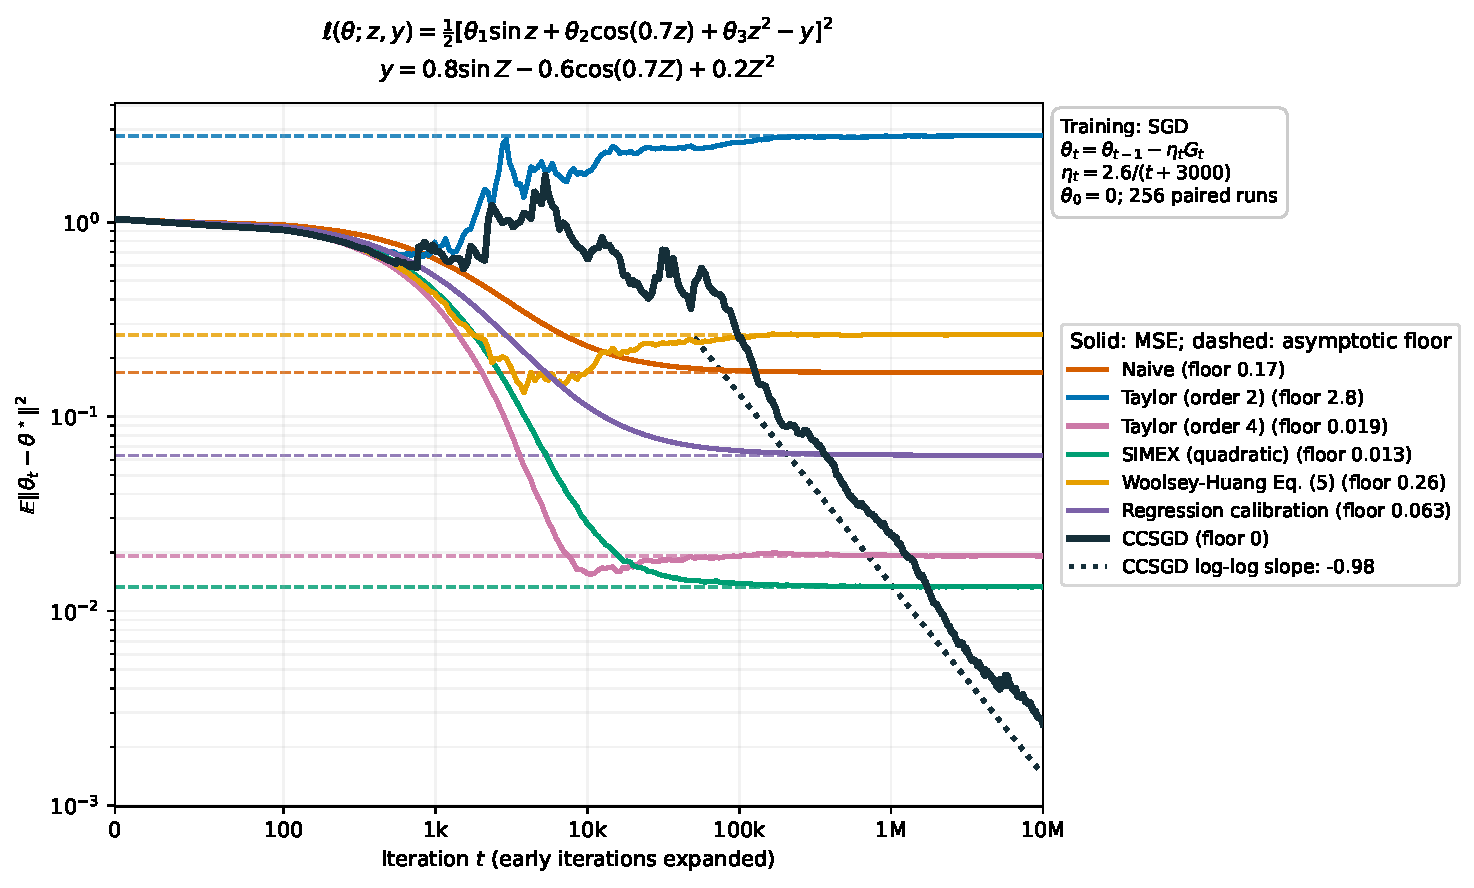
\includegraphics[width=\textwidth]{figure_regression.pdf}
\caption{Parameter MSE averaged over 256 paired runs, starting at
$\theta_0=0$ with $\eta_t=2.6/(t+3000)$.
Dashed lines show the calculated asymptotic squared biases of the specified
baseline updates. Quadratic SIMEX extrapolates three separately optimized
parameter trajectories; its additional Gaussian noise is integrated exactly.
The Woolsey--Huang baseline uses their deterministic Eq.~(5) correction.
The dotted CCSGD guide has fitted log--log slope $-0.978$ over
$5\times10^4\le t\le10^7$.}
\label{fig:nonlinear_regression_mse}
\end{figure}

\subsection{Neural-network regression}
We generate noise-free responses from
\[
Z\sim\operatorname{Unif}[-2,2],\qquad
Y=f_0(Z)=e^{-Z^2}\sin(3Z)+0.3Z^2,
\]
and fit a single-hidden-layer network
\[
h_\theta(z)=c+\sum_{j=1}^{32}a_j\sin(b_jz+d_j),\qquad
\ell(\theta;z,y)=\tfrac12(h_\theta(z)-y)^2,
\]
training all 97 parameters. For each fixed finite parameter vector, the
score is entire and has at most exponential growth in the input; its
Gaussian complex correction is therefore unbiased with finite second
moment. The exponential rate can depend on the input weights; neither
a parameter-independent exponent nor the amplitude control in
\eqref{eq:amplitude_control} is established for this network. Its training
curves are therefore empirical and do not invoke the nonconvex theorem.

We use 8,192 latent training pairs and 4,096 independent clean prediction
pairs, with no validation set. At every minibatch presentation, we generate
fresh $U\sim N(0,0.3^2)$ and observe $W=Z+U$; all methods share these
observations, minibatch indices, and initialization. CCSGD independently
samples $V\sim N(0,0.3^2)$ and computes
\[
\operatorname{Re}\left[(h_\theta(W+iV)-Y)
\nabla_\theta h_\theta(W+iV)\right]
\]
using complex arithmetic and the analytic squared loss, without complex
conjugation. Training uses minibatches of size 128 and
$\eta_t=0.01(1+t/2000)^{-0.6}$.

We compare naive SGD, Taylor corrections of orders two and four,
quadratic SIMEX, the Woolsey--Huang Eq.~(5) correction, and regression
calibration. Taylor corrections differentiate the full score with respect
to its input, holding the response fixed. SIMEX trains separate networks
at additional noise levels $\lambda=0,1,2$ and extrapolates predictions as
$3h^{(0)}-3h^{(1)}+h^{(2)}$. Regression calibration uses the exact
$\mathbb E[Z\mid W]$ under the specified uniform latent distribution.
The prediction set is used only to report
$n_{\rm pred}^{-1}\sum_i(h_{\theta_t}(Z_i)-Y_i)^2$.

\begin{figure}[H]
\centering
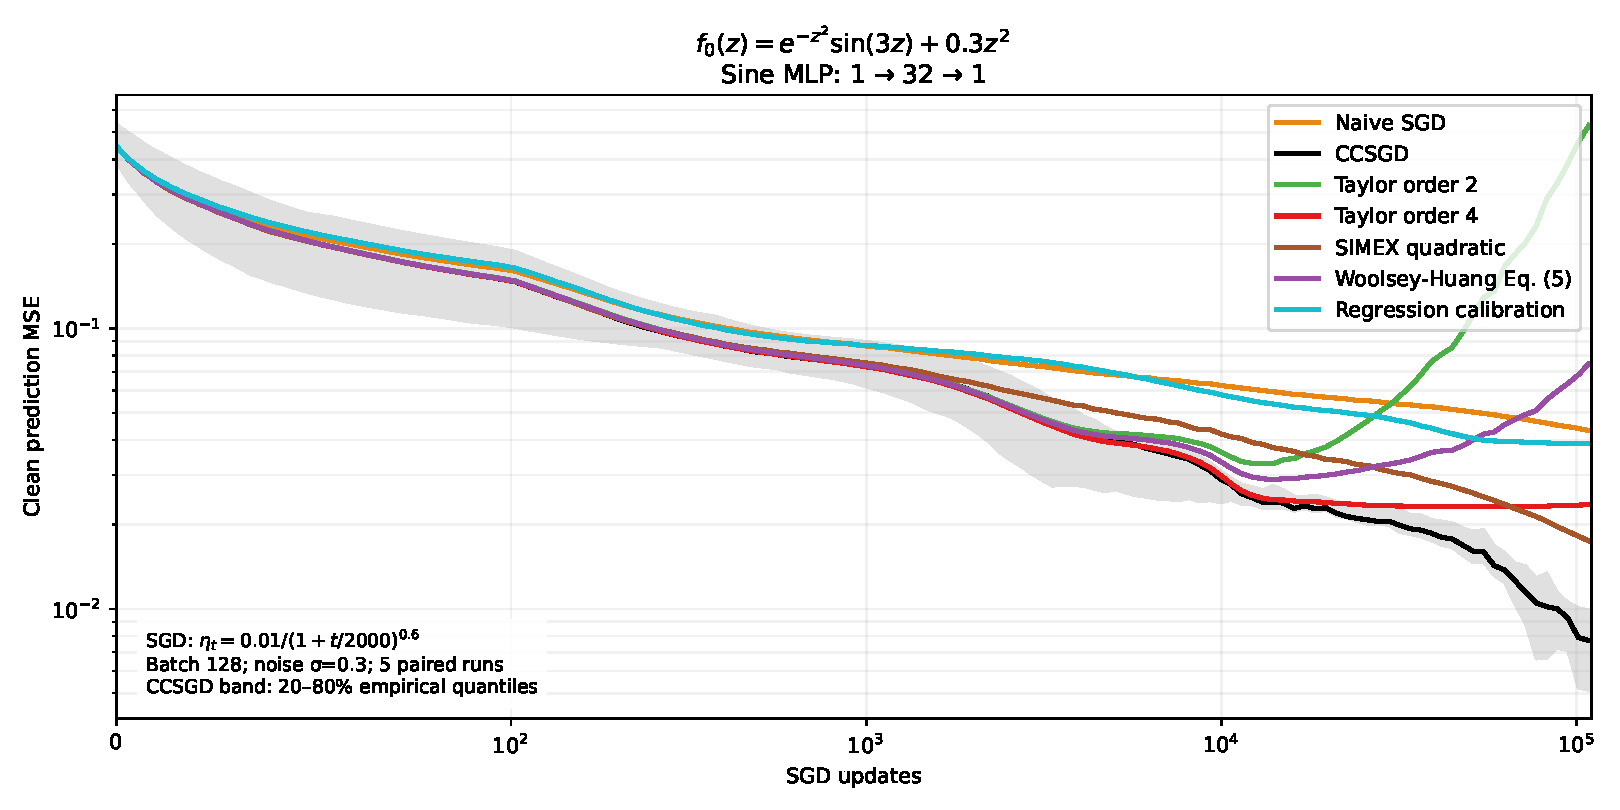
\includegraphics[width=\textwidth]{figure_neural_network.pdf}
\caption{Clean-input prediction MSE averaged over five paired runs.
The shaded CCSGD band gives empirical 20--80\% quantiles.
Training runs for 200,000 updates; the figure displays the trajectory
through $1.1\times10^5$ updates. CCSGD attains lower mean prediction error
than the specified baselines near the displayed endpoint.}
\label{fig:neural_network_mse}
\end{figure}

This experiment targets the clean empirical training objective conditional
on the latent training set. Fresh measurement noise preserves conditional
unbiasedness for that objective; it does not remove finite-sample or
approximation error on the independent prediction set. The methods'
ordering changes during training: at 200,000 updates, mean prediction
MSE is $0.0142$ for CCSGD and $0.0125$ for SIMEX. These results illustrate
finite-time behavior without asserting a zero prediction-error limit.

\section{Further work}
\label{sec:future_work}

\subsection{Noise generalization}
\label{sec:noise_generalization}
The Gaussian perturbation is one instance of a more general conjugate
construction. Our companion manuscript \cite{conjugatecriterion2026}
characterizes symmetric scalar errors $U$ admitting an independent real
variable $V$ such that
\begin{equation}\label{eq:conjugate_transform}
M_U(t)\varphi_V(t)=1,\qquad t\in\mathbb R,
\end{equation}
where $M_U(t)=\mathbb E e^{tU}$ is finite on $\mathbb R$ and
$\varphi_V(t)=\mathbb E e^{itV}$. Existence is equivalent to $1/M_U$
being a characteristic function; the companion manuscript gives Fourier
and moment criteria and constructs the conjugate law. The imaginary
perturbation must follow this law, which generally differs from the
measurement-error law.

\paragraph{Uniform measurement error.}
For $U\sim\operatorname{Unif}[-b,b]$, with known $b>0$,
\[
M_U(t)=\frac{\sinh(bt)}{bt},\qquad
\varphi_V(t)=\frac{bt}{\sinh(bt)},
\]
with both ratios interpreted as $1$ at $t=0$.
The conjugate $V$ has a centered logistic distribution with scale $b/\pi$:
\[
f_V(v)=\frac{\pi}{4b\cosh^2(\pi v/(2b))},\qquad
F_V(v)=\frac{1}{1+e^{-\pi v/b}}.
\]
It can be sampled directly from $R\sim\operatorname{Unif}(0,1)$ via
\begin{equation}\label{eq:uniform_conjugate_sampler}
V=\frac b\pi\log\frac{R}{1-R}.
\end{equation}
Thus a uniform measurement error is corrected by an independent logistic
imaginary perturbation.

\paragraph{Symmetric two-point measurement error.}
For $\mathbb P(U=b)=\mathbb P(U=-b)=1/2$,
\[
M_U(t)=\cosh(bt),\qquad
\varphi_V(t)=\frac1{\cosh(bt)}.
\]
Here $V$ has a scaled hyperbolic-secant distribution:
\[
f_V(v)=\frac{1}{2b\cosh(\pi v/(2b))},\qquad
F_V(v)=\frac2\pi\arctan\!\left(e^{\pi v/(2b)}\right).
\]
An exact sampler is
\begin{equation}\label{eq:binary_conjugate_sampler}
V=\frac{2b}\pi\log\tan\!\left(\frac{\pi R}{2}\right),
\qquad R\sim\operatorname{Unif}(0,1).
\end{equation}
The imaginary perturbation is continuous even though the measurement
error is discrete.

\paragraph{Exact correction and implementation.}
Set $D=U+iV$. Equation~\eqref{eq:conjugate_transform} implies
$\mathbb E D^k=0$ for every integer $k\ge1$
\cite{conjugatecriterion2026}. Hence, for fixed $(\theta,z)$,
\begin{equation}\label{eq:nongaussian_correction}
\mathbb E_{U,V}\operatorname{Re}g^{\mathbb C}(\theta;z+U+iV)
=g(\theta;z)
\end{equation}
for polynomial scores. The identity also holds for entire scores when
\begin{equation}\label{eq:nongaussian_taylor}
\sum_{k=0}^\infty
\frac{\|\partial_z^k g^{\mathbb C}(\theta;z)\|}{k!}
\mathbb E|D|^k<\infty.
\end{equation}
Indeed, this condition permits termwise expectation of the Taylor series;
all nonconstant terms vanish. Thus correction is exact, with no
finite-order truncation. Algorithm~\ref{alg:nongaussian_ccsgd} implements
it using the explicit inverse-distribution samplers above. It requires
the error law and its scale, but not the latent input distribution.

\begin{algorithm}[H]
\caption{CCSGD for uniform or symmetric two-point measurement error}
\label{alg:nongaussian_ccsgd}
\begin{algorithmic}[1]
\Require Initial point $\theta_1$, step sizes $\{\eta_t\}_{t=1}^T$, known error type and scale $b>0$
\For{$t=1,\ldots,T$}
    \State Observe a fresh $W_t=Z_t+U_t$
    \State Draw $R_t\sim\operatorname{Unif}(0,1)$ independently of the observation and the past
    \If{$U_t\sim\operatorname{Unif}[-b,b]$}
        \State $V_t\gets(b/\pi)\log\{R_t/(1-R_t)\}$
    \Else\Comment{$\mathbb P(U_t=\pm b)=1/2$}
        \State $V_t\gets(2b/\pi)\log\tan(\pi R_t/2)$
    \EndIf
    \State $G_t\gets\operatorname{Re}g^{\mathbb C}(\theta_t;W_t+iV_t)$
    \State $\theta_{t+1}\gets\theta_t-\eta_tG_t$
\EndFor
\State \Return $\theta_{T+1}$
\end{algorithmic}
\end{algorithm}
For noise-free responses, the observed response is held fixed during the
complex evaluation, as in Section~\ref{sec:algorithm}. Independent
replicates of $V_t$ may be averaged using the same observation. For
independent input-error coordinates, the construction can also be applied
coordinatewise with independent conjugate perturbations, subject to the
corresponding multivariate integrability condition.

\paragraph{Moment conditions for optimization.}
Unlike a Gaussian conjugate, these conjugates have exponential moments
only below a finite threshold. Specifically,
\[
\mathbb E e^{s|V|}<\infty\quad\Longleftrightarrow\quad 0\le s<\lambda,
\qquad
\lambda=
\begin{cases}
\pi/b, & U\sim\operatorname{Unif}[-b,b],\\
\pi/(2b), & \mathbb P(U=\pm b)=1/2.
\end{cases}
\]
Under the derivative envelope~\eqref{eq:parameter_envelope}, the strict
condition $a<\lambda$ suffices for
\eqref{eq:nongaussian_taylor}: the score has exponential growth of any
rate slightly larger than $a$, and the conjugate has an exponential
moment at a still larger rate. If $2a<\lambda$, boundedness of $U$ gives
\[
K_a=\mathbb E e^{2a|Z|}\,
\mathbb E[|D|^2e^{2a|D|}]<\infty.
\]
Together with the clean sampling and amplitude bounds, the same argument
as in Section~\ref{sec:main_results} yields the relative variance
condition~\eqref{eq:relative_variance}. For the CLTs, choose $\delta>0$
with $(2+\delta)a<\lambda$; the higher-moment proof then applies as well.
Thus the optimization analysis transfers when these moment conditions
and the corresponding objective and covariance assumptions are verified.
Polynomial scores satisfy the required input moment conditions for both
pairs. Arbitrary entire scores still require growth control, and random
responses require the corresponding joint moment bounds.

\subsection{Function generalization}
Exact Gaussian correction restricts the admissible score class. In the scalar Gaussian location model with positive noise
variance, Stefanski \cite{stefanski1989} shows that a target admitting an
integrable unbiased estimator for every real mean must extend to an entire
function. Applied componentwise at fixed $\theta$, this rules out globally
exact unbiased correction of non-entire scores in that setting.
Entire analyticity alone does not ensure the integrability required by
CCSGD; growth control remains essential. For non-entire scores, a natural
direction is approximate or regularized correction with explicit bias,
variance, and optimization-error bounds. With singular $\Omega$, the
analyticity restriction concerns the directions affected by noise.

\appendix
\section{Proofs of the main results}\label{app:proofs}

\subsection{Proof of Lemma~\ref{lem:exact_correction}}
\begin{proof}
Fix $\theta$ and $z\in\mathbb R^d$, and put $C=U+iV$.
The fundamental theorem of calculus and the exponential envelope give, for every $q\in\mathbb C^d$,
\begin{equation}\label{eq:appendix_score_envelope}
\|g^{\mathbb C}(\theta;q)-g(\theta;0)\|
\le M(\theta)\|q\|e^{a\|q\|}.
\end{equation}
Since $C$ is complex Gaussian, its norm has exponential moments of every linear order. Thus $g^{\mathbb C}(\theta;z+C)$ is absolutely integrable. The same bound permits exchange of the expectation and angular integral below.

For every $\phi\in[0,2\pi]$, the real pair
\[
(\operatorname{Re}(e^{i\phi}C),\operatorname{Im}(e^{i\phi}C))
=(U\cos\phi-V\sin\phi,\;U\sin\phi+V\cos\phi)
\]
has the same centered Gaussian law as $(U,V)$: its covariance is $\operatorname{diag}(\Omega,\Omega)$. Hence $e^{i\phi}C\overset{d}=C$. On the other hand, for each fixed $c\in\mathbb C^d$, the one-variable function $s\mapsto g^{\mathbb C}(\theta;z+sc)$ is entire. Cauchy's mean-value formula, applied componentwise, gives
\[
\frac{1}{2\pi}\int_0^{2\pi}
g^{\mathbb C}(\theta;z+e^{i\phi}c)\,d\phi
=g^{\mathbb C}(\theta;z)=g(\theta;z).
\]
Taking expectation over $C$ and using rotational invariance yields
\[
\mathbb E\,g^{\mathbb C}(\theta;z+C)
=\mathbb E\!\left[\frac{1}{2\pi}\int_0^{2\pi}
g^{\mathbb C}(\theta;z+e^{i\phi}C)\,d\phi\right]
=g(\theta;z).
\]
Taking real parts proves the first claim. For the second, condition on $\mathcal F_{t-1}$, apply the first claim conditional on $Z_t$, and then average over $Z_t$. Predictability and the assumed interchange of gradient and expectation give $\nabla F(\theta_t)$.
\end{proof}

\subsection{Reduction to classical SGD noise conditions}
\begin{proof}
Put $D=U+iV$. The fundamental theorem of calculus gives
\[
\|\operatorname{Re}g^{\mathbb C}(\theta;Z+D)-g(\theta;Z)\|
\le M(\theta)\|D\|e^{a(\|Z\|+\|D\|)}.
\]
Independence of $Z$ and $D$ gives
$\mathbb E\|\Delta(\theta)\|^2\le K_aM(\theta)^2$.
Equation~\eqref{eq:amplitude_control} then gives the correction-error
bound in the main text.
Sub-Gaussian vectors in finite dimension have exponential moments of their
norm of every linear order; the same holds for the Gaussian pair $(U,V)$,
regardless of whether $\Omega$ is singular. Hence $K_a<\infty$.
Conditioning first on $Z_t$ and using exact correction shows that
$\Delta_t$ is orthogonal in $L^2$ to
$g(\theta_t;Z_t)-\nabla F(\theta_t)$. This proves
\eqref{eq:relative_variance}. In particular,
\begin{equation}\label{eq:score_second_moment}
\mathbb E_t\|G_t\|^2
\le\sigma^2+(1+\rho)\|\nabla F(\theta_t)\|^2.
\end{equation}
For the CLTs, stronger moments follow from the same input bound.
Set $b_a(q)=\|q\|e^{a\|q\|}$ and $Q=Z+U+iV$. Centering cancels
$g(\theta;0)$ and gives
\[
\|G(\theta)-\nabla F(\theta)\|
\le M(\theta)\bigl[b_a(Q)+\mathbb E b_a(Z)\bigr].
\]
The bracket has moments of every finite order. Hence, for every $r\ge2$,
\begin{equation}\label{eq:higher_noise_moments}
\mathbb E_t\|\xi_t\|^r\le C_r M(\theta_t)^r
\le C_r\bigl(A+B\|\nabla F(\theta_t)\|^2\bigr)^{r/2},
\end{equation}
where $C_r$ is deterministic and finite. Under the strong convexity and
smoothness conditions used for the CLTs, almost-sure convergence gives
\[
\sup_t\|\nabla F(\theta_t)\|<\infty\quad\text{almost surely}.
\]
Thus the conditional higher moments are bounded along each convergent
trajectory by a finite random constant. On a fixed neighborhood of
$\theta^*$ the bound is deterministic, since
$\|\nabla F(\theta)\|\le L\|\theta-\theta^*\|$.
These bounds supply the Lindeberg control below without a global
uniform bound on $M$ or a moment assumption on the corrected score.
\end{proof}

\subsection{Convex convergence}
\begin{proof}
Write $e_t=\theta_t-\theta^*$ and $f_t=F(\theta_t)-F(\theta^*)$.
For a convex, $L$-smooth function,
\[
\langle\nabla F(\theta_t),e_t\rangle
\ge f_t+\frac1{2L}\|\nabla F(\theta_t)\|^2.
\]
Expanding the squared distance, using unbiasedness and
\eqref{eq:score_second_moment}, gives
\[
\mathbb E_t\|e_{t+1}\|^2
\le\|e_t\|^2-2\eta_tf_t
+\bigl((1+\rho)\eta_t^2-\eta_t/L\bigr)
\|\nabla F(\theta_t)\|^2+\sigma^2\eta_t^2.
\]
The gradient term is nonpositive under the stated step-size bound.
Taking expectations, summing, and applying convexity to the weighted
average proves the displayed bound. The rates follow from
$\sum_t\eta_t^2<\infty$ and the growth of $\sum_{t\le T}\eta_t$.
\end{proof}

\subsection{Strong convexity and MSE}
\begin{proof}
Write $e_t=\theta_t-\theta^*$. Strong convexity and smoothness give
$\langle\nabla F(\theta_t),e_t\rangle\ge\mu\|e_t\|^2$ and
$\|\nabla F(\theta_t)\|\le L\|e_t\|$. Hence
\begin{equation}\label{eq:strong_recursion}
\mathbb E_t\|e_{t+1}\|^2
\le\bigl(1-2\mu\eta_t+(1+\rho)L^2\eta_t^2\bigr)\|e_t\|^2
+\sigma^2\eta_t^2.
\end{equation}
This inequality first ensures finite second moments at every finite time.
The Robbins--Siegmund theorem \cite{robbinssiegmund1971}, applied with
summable coefficients $(1+\rho)L^2\eta_t^2$ and $\sigma^2\eta_t^2$,
then shows that $\|e_t\|^2$ converges almost surely and
$\sum_t\eta_t\|e_t\|^2<\infty$. Since $\sum_t\eta_t=\infty$,
the limit is zero.

For the rates, put $u_t=\mathbb E\|e_t\|^2$, $h_t=t+\gamma$,
$A=2\mu c$, $B=(1+\rho)L^2c^2$, and $D=\sigma^2c^2$.
Taking expectations gives
\begin{equation}\label{eq:mse_scalar}
u_{t+1}\le(1-Ah_t^{-\alpha}+Bh_t^{-2\alpha})u_t
+Dh_t^{-2\alpha}.
\end{equation}
If $\alpha<1$, choose $N$ so that the coefficient is nonnegative and
at most $1-(A/2)h_t^{-\alpha}$ for $t\ge N$.
Choose $M\ge4D/A$ with $u_N\le Mh_N^{-\alpha}$.
Increasing $N$ if needed, $h_t^{1-\alpha}\ge4\alpha/A$.
The induction hypothesis $u_t\le Mh_t^{-\alpha}$ then implies
\[
u_{t+1}\le Mh_t^{-\alpha}-\frac{AM}{4}h_t^{-2\alpha}
\le M(h_t+1)^{-\alpha},
\]
where the last inequality uses
$h^{-\alpha}-(h+1)^{-\alpha}\le\alpha h^{-\alpha-1}$.
After adjusting $M$ at this fixed starting index, induction proves
$u_t=O(t^{-\alpha})$.

If $\alpha=1$, choose $N$ so that $q_j=1-A/h_j+B/h_j^2>0$ for
$j\ge N$. Since $\log q_j=-A/h_j+O(h_j^{-2})$,
\[
\prod_{j=s}^{t-1}q_j\le C(h_s/h_t)^A\qquad(t>s\ge N),
\]
with a constant independent of $s,t$. Iterating \eqref{eq:mse_scalar}
therefore gives
\[
u_t\le C h_t^{-A}
\left(h_N^Au_N+D\sum_{s=N}^{t-1}h_s^{A-2}\right).
\]
The sum is $O(t^{A-1})$ for $A>1$, $O(\log t)$ for $A=1$,
and $O(1)$ for $A<1$. These are the three asserted rates, and all
converge to zero.
\end{proof}

\subsection{Preparatory estimates for the central limit theorems}
\label{app:clt_preparation}
Throughout the CLT proofs, write
$\bar e_T=T^{-1}\sum_{t=1}^Te_t=\bar\theta_T-\theta^*$,
and put $h=\lambda_{\min}(H)>0$ and
\[
r(e)=\nabla F(\theta^*+e)-He.
\]
Local Lipschitz continuity of the Hessian gives a radius $\varepsilon_0>0$
and a constant $C_r$ such that
$\|r(e)\|\le C_r\|e\|^2$ for $\|e\|\le\varepsilon_0$.
Globally, smoothness gives $\|r(e)\|\le(L+\|H\|)\|e\|$.

\paragraph{Localization.}
Choose $0<\varepsilon\le\varepsilon_0$ and define
$\tau_N=\inf\{t\ge N:\|e_t\|>\varepsilon\}$, with
$\inf\varnothing=\infty$. Almost-sure convergence implies
\begin{equation}\label{eq:localization_probability}
\mathbb P(\tau_N<\infty)\longrightarrow0\qquad(N\to\infty).
\end{equation}
For $\alpha<1$, the global MSE bound yields
\[
\mathbb E[\|r(e_t)\|\mathbf1_{\{\tau_N>t\}}]
\le C\,t^{-\alpha}.
\]
For $\alpha=1$, the local spectral condition $ch>1/2$ permits a choice
$m\in(1/(2c),h)$ and a sufficiently small $\varepsilon$ such that
$\langle\nabla F(\theta^*+e),e\rangle\ge m\|e\|^2$
on this ball. The event $\{\tau_N>t\}$ is measurable with respect to
$\mathcal F_{t-1}$. Setting
$v_t=\mathbb E[\|e_t\|^2\mathbf1_{\{\tau_N>t\}}]$, discarding
paths that exit at the next step gives
\[
v_{t+1}\le(1-2m\eta_t+(1+\rho)L^2\eta_t^2)v_t+\sigma^2\eta_t^2.
\]
The preceding scalar comparison, with $2mc>1$, gives
\begin{equation}\label{eq:localized_remainder}
v_t=O_N(t^{-1}),\qquad
\mathbb E[\|r(e_t)\|\mathbf1_{\{\tau_N>t\}}]=O_N(t^{-1}).
\end{equation}
Here constants may depend on the fixed starting index $N$.
We first take the iteration horizon to infinity and then let $N\to\infty$
in \eqref{eq:localization_probability}. Thus a remainder that vanishes
on these localized paths is $o_p(1)$ for the original process.

\paragraph{Matrix products.}
For $b\ge a$, let $P_{a,b}=\prod_{j=a}^b(I-\eta_jH)$, and set
$P_{a,b}=I$ when $a>b$. Choose $N$ large enough that
$\eta_j\|H\|<1$ for $j\ge N$. Spectral decomposition gives
\begin{equation}\label{eq:product_bounds}
\begin{aligned}
\|P_{s+1,t-1}\|&\le
\exp\left(-h\sum_{j=s+1}^{t-1}\eta_j\right), &&\alpha<1,\\
\|P_{s+1,t-1}\|&\le C_\nu
\left(\frac{s+\gamma}{t+\gamma}\right)^\nu,
&&\alpha=1,\quad 0<\nu<ch,
\end{aligned}
\end{equation}
for $t>s\ge N$. For the second bound, apply
$\log(1-c\lambda/(j+\gamma))=-c\lambda/(j+\gamma)+O(j^{-2})$
to each eigenvalue $\lambda$ of $H$ and sum over $j$.

\paragraph{A common martingale CLT argument.}
Equation~\eqref{eq:higher_noise_moments}, almost-sure convergence, and covariance continuity imply, for some
$\delta>0$,
\[
\mathbb E_t\xi_t=0,\qquad
\sup_t\mathbb E_t\|\xi_t\|^{2+\delta}\le C_\delta(\omega)<\infty,\qquad
S(\theta_t)\longrightarrow S_*\quad\text{almost surely}.
\]
Let $D_{T,s}$ be deterministic matrix weights such that
\begin{equation}\label{eq:weight_conditions}
\max_s\|D_{T,s}\|\to0,\qquad
\sup_T\sum_s\|D_{T,s}\|^2<\infty,\qquad
\sum_sD_{T,s}S_*D_{T,s}^\top\to\Sigma.
\end{equation}
Splitting the sum at a fixed index and then sending that index to infinity
shows that replacing $S_*$ by $S(\theta_s)$ changes the last limit by
$o(1)$ almost surely. For each $\epsilon>0$, conditional Lindeberg follows
from
\[
\sum_s\mathbb E_s\!\left[
\|D_{T,s}\xi_s\|^2\mathbf1_{\{\|D_{T,s}\xi_s\|>\epsilon\}}\right]
\le C_\delta(\omega)\epsilon^{-\delta}
\max_s\|D_{T,s}\|^\delta\sum_s\|D_{T,s}\|^2\longrightarrow0\quad\text{almost surely}.
\]
The martingale array CLT and the Cram\'er--Wold argument therefore give
$\sum_sD_{T,s}\xi_s\Rightarrow N(0,\Sigma)$
\cite[Chapter~3]{hallheyde1980}. This verifies explicitly the probabilistic
conditions used in the following two proofs.

\subsection{Last-iterate fluctuations}
\begin{proof}[Proof of Theorem~\ref{thm:last_clt}]
The exact recursion, started at a fixed sufficiently large $N$, is
\begin{equation}\label{eq:linear_representation}
e_t=P_{N,t-1}e_N-
\sum_{s=N}^{t-1}\eta_sP_{s+1,t-1}\xi_s-
\sum_{s=N}^{t-1}\eta_sP_{s+1,t-1}r(e_s).
\end{equation}
We verify directly the linearization and covariance limits underlying
the stochastic approximation CLT of Fabian \cite{fabian1968}.

If $\alpha<1$, the first term multiplied by $t^{\alpha/2}$ vanishes
by \eqref{eq:product_bounds}. On localized paths, the expected norm of
the scaled last term is bounded by
\[
C t^{\alpha/2}\sum_{s=N}^{t-1}\eta_s
\exp\left(-h\sum_{j=s+1}^{t-1}\eta_j\right)s^{-\alpha}
=O(t^{-\alpha/2}).
\]
To see this, split at $t/2$. The earlier terms have an exponentially
small factor $e^{-c_1t^{1-\alpha}}$; for the later terms,
$s^{-\alpha}\le C t^{-\alpha}$ and the remaining weighted geometric
sum is bounded. Localization then makes this term $o_p(1)$.

Set $D_{t,s}=t^{\alpha/2}\eta_sP_{s+1,t-1}$.
The same product bound gives
$\max_s\|D_{t,s}\|=O(t^{-\alpha/2})$ and
$\sum_s\|D_{t,s}\|^2=O(1)$.
On the window $t-s=O(\eta_t^{-1})$, uniformly on bounded rescaled
intervals, $\eta_s/\eta_t\to1$ and
$P_{s+1,t-1}=e^{-H\eta_t(t-s)}+o(1)$.
Riemann summation, using $t^\alpha\eta_t\to c$, gives
\[
\sum_{s=N}^{t-1}D_{t,s}S_*D_{t,s}^\top
\longrightarrow c\int_0^\infty e^{-Hv}S_*e^{-Hv}\,dv.
\]
The omitted tail beyond $t-s>R/\eta_t$ is bounded by $Ce^{-c_2R}$
after the negligible range $s<t/2$ is removed. This justifies sending
$R\to\infty$. The common martingale argument proves the first CLT.

If $\alpha=1$, fix $\nu\in(1/2,\min\{ch,1\})$.
The scaled initial term is $O_p(t^{1/2-\nu})=o_p(1)$.
By \eqref{eq:localized_remainder}, the localized expected norm of the
scaled nonlinear term is at most
\[
C_N t^{1/2-\nu}\sum_{s=N}^{t-1}s^{\nu-2}
=O_N(t^{1/2-\nu})=o(1).
\]
Set $D_{t,s}=\sqrt t\,\eta_sP_{s+1,t-1}$. Then
$\|D_{t,s}\|\le C t^{-1/2}(s/t)^{\nu-1}$, so the first two
conditions in \eqref{eq:weight_conditions} hold. Uniformly for
$s/t$ in compact subsets of $(0,1]$,
\[
\sqrt t\,D_{t,s}\longrightarrow c\,u^{cH-I}
\quad\text{when }s/t\to u.
\]
The squared-weight sum over $N\le s\le\varepsilon t$ is bounded by
$C\varepsilon^{2\nu-1}$. Hence Riemann summation gives
\[
\sum_{s=N}^{t-1}D_{t,s}S_*D_{t,s}^\top
\longrightarrow c^2\int_0^1u^{cH-I}S_*u^{cH-I}\,du.
\]
The martingale argument proves the endpoint CLT.

Finally, the first integral covariance solves
$H\Sigma_c+\Sigma_cH=cS_*$. In the second integral, the substitution
$u=e^{-v}$ gives
$c^2\int_0^\infty e^{-(cH-I/2)v}S_*e^{-(cH-I/2)v}\,dv$,
which solves the stated endpoint equation. Positive definiteness of
$H$ and $cH-I/2$, respectively, gives uniqueness and positive
semidefiniteness of these solutions.
\end{proof}

\subsection{Polyak--Ruppert averaging}
\begin{proof}[Proof of Theorem~\ref{thm:pr_clt}]
Suppose first that $\alpha<1$. Summing
$He_t=(e_t-e_{t+1})/\eta_t-\xi_t-r(e_t)$ from $N$ to $T$ gives
\[
H\sum_{t=N}^Te_t=-\sum_{t=N}^T\xi_t-
\sum_{t=N}^Tr(e_t)+R_{N,T},
\]
where summation by parts yields
\[
R_{N,T}=\frac{e_N}{\eta_N}-\frac{e_{T+1}}{\eta_T}
+\sum_{t=N+1}^T(\eta_t^{-1}-\eta_{t-1}^{-1})e_t.
\]
Since $\mathbb E\|e_t\|=O(t^{-\alpha/2})$ and
$\eta_t^{-1}-\eta_{t-1}^{-1}=O(t^{\alpha-1})$,
\[
T^{-1/2}\mathbb E\|R_{N,T}\|
=O_N(T^{-1/2})+O(T^{(\alpha-1)/2})=o(1).
\]
The localized nonlinear sum, divided by $\sqrt T$, has expected norm
at most
\[
C T^{-1/2}\sum_{t=N}^Tt^{-\alpha}=O(T^{1/2-\alpha})=o(1).
\]
Removing localization and the finite initial segment gives the classical
averaging representation
\cite{polyakjuditsky1992}
\[
\sqrt T\,\bar e_T=-H^{-1}\frac1{\sqrt T}\sum_{t=1}^T\xi_t+o_p(1).
\]
Taking $D_{T,s}=H^{-1}/\sqrt T$ in
\eqref{eq:weight_conditions} proves the first assertion.

For $\alpha=1$, use the product representation
\eqref{eq:linear_representation} and define
\[
B_{T,s}=\eta_s\sum_{t=s+1}^TP_{s+1,t-1},\qquad N\le s\le T,
\]
Then
\[
\sqrt T\,\bar e_T=-\frac1{\sqrt T}\sum_{s=N}^{T-1}B_{T,s}\xi_s
-\frac1{\sqrt T}\sum_{s=N}^{T-1}B_{T,s}r(e_s)+I_{N,T},
\]
where $B_{T,T}=0$ and $I_{N,T}$ contains the finite initial segment and the propagated
initial value. For $\nu\in(1/2,\min\{ch,1\})$,
\eqref{eq:product_bounds} implies
\begin{equation}\label{eq:averaging_weight_bound}
\|B_{T,s}\|\le C s^{\nu-1}\sum_{t=s+1}^Tt^{-\nu}
\le C(s/T)^{\nu-1},\qquad
I_{N,T}=O_p(T^{1/2-\nu}).
\end{equation}
By \eqref{eq:localized_remainder}, the localized nonlinear sum is
bounded in expected norm by
\[
\frac{C_N}{\sqrt T}\sum_{s=N}^{T-1}(s/T)^{\nu-1}s^{-1}
=O_N(T^{1/2-\nu})=o(1).
\]
Thus both remainders vanish in probability.

To identify the weights, the eigenvalue expansion used in
\eqref{eq:product_bounds} gives, uniformly when
$\varepsilon T\le s<t\le T$,
\[
P_{s+1,t-1}=((s+\gamma)/(t+\gamma))^{cH}+O_\varepsilon(T^{-1}).
\]
Consequently, uniformly on compact subsets of $(0,1]$,
\[
B_{T,\lfloor Tu\rfloor}\longrightarrow
K_c(u)=c\,u^{cH-I}\int_u^1v^{-cH}\,dv.
\]
Both $B_{T,s}$ and $K_c(s/T)$ satisfy the bound
$C(s/T)^{\nu-1}$. In particular,
\[
\frac1T\sum_{N\le s\le\varepsilon T}
\bigl(\|B_{T,s}\|^2+\|K_c(s/T)\|^2\bigr)
\le C\varepsilon^{2\nu-1}.
\]
Compact convergence and this bound establish
\begin{equation}\label{eq:kernel_l2}
\frac1T\sum_{s=N}^{T-1}\|B_{T,s}-K_c(s/T)\|^2\longrightarrow0.
\end{equation}
The relative variance bound, smoothness, and the strong-convexity MSE
estimate imply $\sup_s\mathbb E\|\xi_s\|^2<\infty$.
Martingale orthogonality therefore shows that
replacing $B_{T,s}$ by $K_c(s/T)$ in the noise sum produces an
$o_{L^2}(1)$ error. The finitely many terms with $s<N$ vanish because
$T^{-1/2}\|K_c(s/T)\|=O(T^{1/2-\nu})$ for fixed $s$.
We have therefore proved
\[
\sqrt T\,\bar e_T=-\frac1{\sqrt T}\sum_{s=1}^{T-1}K_c(s/T)\xi_s+o_p(1).
\]
For $D_{T,s}=T^{-1/2}K_c(s/T)$,
\eqref{eq:averaging_weight_bound} gives vanishing maximum weight and a
bounded squared-weight sum. The same compact/tail decomposition gives
\[
\sum_{s=1}^{T-1}D_{T,s}S_*D_{T,s}^\top
\longrightarrow\int_0^1K_c(u)S_*K_c(u)^\top\,du.
\]
The common martingale CLT argument completes the proof.
\end{proof}

\subsection{Nonconvex stationarity}
\begin{proof}
Smoothness, unbiasedness, and \eqref{eq:score_second_moment} give
\[
\mathbb E_tF(\theta_{t+1})
\le F(\theta_t)-\eta_t\left(1-\tfrac L2(1+\rho)\eta_t\right)
\|\nabla F(\theta_t)\|^2+\tfrac L2\sigma^2\eta_t^2.
\]
The stated step-size bound makes the descent coefficient at least
$\eta_t/2$. Taking expectations, summing, and using
$F(\theta_{T+1})\ge F_{\inf}$ proves the bound and the asserted rates.
\end{proof}


\subsection{Moment bounds for nonlinear-feature regression}
\label{app:regression}
For the regression model in Section~\ref{sec:experiments}, write
$Q=Z+U+iV$, $\theta^*=\theta_{\rm true}$, and
\[
A=\operatorname{Re}\{\psi(Q)\psi(Q)^\top\},\qquad
b=Y\operatorname{Re}\psi(Q),\qquad
H=\mathbb E[\psi(Z)\psi(Z)^\top].
\]
The corrected gradient is $G(\theta)=A\theta-b$.
Gaussian tails, the polynomial growth of $Y$, and the exponential growth
of the sine and cosine factors imply that $A$ and $b$ have moments of
every finite order. Conditional exact correction gives
$\mathbb EA=H$ and $\mathbb Eb=H\theta^*$.
The functions $\sin z$, $\cos(0.7z)$, and $z^2$ are linearly independent
on $\mathbb R$, and the latent density is positive everywhere.
Consequently $H\succ0$ and
\[
F(\theta)=\tfrac12(\theta-\theta^*)^\top H(\theta-\theta^*).
\]
Putting $e=\theta-\theta^*$ and $\mu=\lambda_{\min}(H)$, we obtain
\[
\xi(\theta)=(A-H)e+(A\theta^*-b),\qquad
\mathbb E\|\xi(\theta)\|^2
\le 2\mathbb E\|A\theta^*-b\|^2
+2\mathbb E\|A-H\|_{\rm op}^2\|e\|^2.
\]
Since $\|e\|\le\mu^{-1}\|\nabla F(\theta)\|$, this derives
\eqref{eq:relative_variance} directly from the data and score moments,
with finite constants. This argument verifies the required variance
condition for the joint response model, whose response-dependent envelope
is discussed in Section~\ref{sec:algorithm}. The proof of
Theorem~\ref{thm:strong_convex} therefore applies.
Here $\mu\approx0.382$ and $c=2.6$, so $2\mu c>1$ and the theoretical
MSE rate is $O(t^{-1})$.
The numerical value of $\mu$ is obtained from population quadrature.

\section{Experimental details}
\label{app:experiment_details}

\paragraph{Baseline updates.}
Both experiments use scalar inputs. Write $s^2$ for the measurement-noise
variance and suppress the iteration index. Taylor corrections use
\[
G_{\mathrm{T2}}=g(\theta;W,Y)-\frac{s^2}{2}\partial_w^2g(\theta;W,Y),
\qquad
G_{\mathrm{T4}}=G_{\mathrm{T2}}+
\frac{s^4}{8}\partial_w^4g(\theta;W,Y),
\]
with the response held fixed. The deterministic Woolsey--Huang baseline
uses $\operatorname{Re}g^{\mathbb C}(\theta;W+is,Y)$; CCSGD instead
samples $V\sim N(0,s^2)$ at every update. Regression calibration substitutes
the exact conditional mean $\mathbb E[Z\mid W]$ under the stated latent law.
Quadratic SIMEX trains three models with additional Gaussian noise
variances $\lambda s^2$, $\lambda=0,1,2$. It extrapolates parameters in
nonlinear-feature regression and predictions in neural-network regression,
with weights $(3,-3,1)$. In the first experiment its additional-noise
expectation is integrated analytically; in the second it is sampled.
These comparisons use common data streams and step-size schedules;
SIMEX uses three training trajectories, so update counts do not equalize
computational cost.

\paragraph{Population reference lines.}
In nonlinear-feature regression, each direct baseline has a population
score $H_k\theta-r_k$. The dashed line is
$\|H_k^{-1}r_k-\theta^*\|^2$; for SIMEX it is the squared distance between
the extrapolation of the three population minimizers and $\theta^*$.
We evaluate $H_k$ by 160-node Gauss--Hermite quadrature and $r_k$ by
$128\times128$ joint quadrature over $(Z,U)$, retaining the dependence
between $Y$ and $W$. Thus the reference lines are numerical evaluations
of population squared biases, not fits to the simulated trajectories or
lower bounds at every finite iteration.

\bibliographystyle{plain}
\bibliography{references}
\end{document}
